%Chapter 3
\chapter{Developing a simulation methodology}
\thispagestyle{empty}
\vspace{38em}
\hrulefill
\\
\enquote*{\textit{Quote.}} - Somebody\\
\newpage
\section{Introduction}
This chapter details the implementation methodology of simulations to optimize mining compressed air systems. The methodology discussed in this chapter will utilize insights from previous studies. Improving on shortcomings discussed in section \ref{Shortcomings of previous work}.
\par 
Implementation of a simulation is split into three steps. Firstly, an investigation on the specific air network to is performed. The data acquired from this investigation is then utilized to develop and verify a simulation model. Finally scenarios are implemented using the simulations and the results are quantified and ranked. A simulation  report is then produced and passed to the mine.
\section{System investigation method}
	\subsection{Preamble}
		Developing a detailed simulation model of a compressed air network requires thorough comprehension of the inner workings of the system. This section will discuss the investigations needed to obtain the required understanding.
	\subsection{Data acquisition and verification} % 
		- Layouts, data from SCADA Instrumentation, etc.\\
		- Verification of accurate data - Gous article
	\subsection{Solutions to unavailable data}
		Parameters that are required to develop the simulation model, such as flows, pressures, may not be actively logged by mine systems. To obtain this data it is necessary to investigate alternative sources. At points where instrumentation is absent, estimations can be made from assumptions made using instrumentation on the network or spot inspections.
		\par 
		Air network specifications such as piping sizes, technical layouts, major leak locations or specifications is often outdated or not recorded. Critical data should be obtained through audits and inspections of the system. If manual inspection is not possible, estimations should be made using the available data or approximation techniques discussed in literature. %\texttt{REMEMBER TO REFERENCE\\ SPECIFIC LOCATION LITERATURE}.
	\subsection{Mining schedule}
		A crucial aspect to developing an accurate model of a mining compressed air system is understanding the the operational philosophy of the mine. The schedule for operations such as drilling,  blasting or cleaning can have a major impact on compressed air requirements at different times of the day. By utilizing the operational schedule, simulation scenarios can be optimized for the air requirements throughout the day.
	\subsection{Summary}
		
\section{Model development and verification}
	\subsection{Preamble}
	Compressed air networks are comprised of components such as compressors, valves, pipes, etc. This section will discus the development, calibration and verification of component models that make up a compressed air simulation is. 
	\subsection{Compressed air component models}
		\subsubsection{Air pipes}
		Pressure losses occur over compressed air networks due to friction in the pipe, these losses should be taken into account in the simulation for large piping sections. A pipe model is used to account for these losses which are defined by the \textit{Darcy-Weisbach equation}\footnote{ B. Glenn, \enquote*{The Darcy–Weisbach Equation,}[Online] \url{https://bae.okstate.edu/faculty-sites/Darcy/DarcyWeisbach/Darcy-WeisbachEq.htm}, [Accessed 20-05-2017]}:
		$$\Delta P = \frac{f  L \rho V^2}{2 D}$$
		Where the pressure difference $\Delta P $ is a function of:\\
		\begin{tabular}{p{1.3cm}p{13cm}}
		$f$ & Friction coefficient  \\
		$L$ & Pipe length ($m$) \\
		$D$ & Pipe diameter ($m$) \\
		$\rho$ & Air density ($kg/m^3$)\\	
		$V$ & Average velocity ($m/s$) \\
		\end{tabular} \\
		The pipe component can be used as a valve by controlling the open fraction between 0 and 1. Modelling the valve flow characteristics is discussed in \ref{Controllers} \textit{Controllers}.
		\subsubsection{Ambient conditions}
		Ambient air condition underground and on surface can effect the performance of the network [\texttt{Citation needed}]. Pressure and temperature increases with depth as a result of auto compression and rock face temperature [\texttt{Citation needed}]. Therefore it is important to take into account conditions for the boundary conditions at each mining level or area where compressed air is used.   
		\subsubsection{Compressors}
		Three compressor models were investigated, each with varying complexity. The models are: air compressor, dynamic compressor and positive displacement compressor. The air compressor is a general, simplified model. It requires minimal user inputs by making several assumptions. This is useful when parameters for a compressor are not available. Or when doing a quick preliminary simulation. However it is not ideal for detailed simulations which require more precision. 
		\par 
		The dynamic compressor components are is more complex, taking into account factors such as heat generated by \gls{polyCof} and inefficiencies within the process. Hence the model can be used more accurately and for more complex simulations then the general compressor model. However, it should be noted that the dynamic compressor is simplified by several assumptions, for example, a constant efficiency at varying loads. 
		\par 	 
		For most scenarios, the dynamic compressor model is most suitable. This component is modelled by fitting a quadratic curve through three points of operation to obtain an equation for corrected mass flow as a function of the pressure ratio. This characteristic curve of compressor  as shown in figure \ref{fig: Compressor Curve} can be accurately estimated even when only one data point is available by making approximations for the zero flow and pressure points on the curve. Once the flow characteristics of the compressors are set, the efficiency and \gls{polyCof} parameters are calibrated such that the output power and air temperature match the actual or estimated outputs of the compressor.
		
		\begin{figure}[h]
			\centering
			\fbox{% GNUPLOT: LaTeX picture with Postscript
\begingroup
  \makeatletter
  \providecommand\color[2][]{%
    \GenericError{(gnuplot) \space\space\space\@spaces}{%
      Package color not loaded in conjunction with
      terminal option `colourtext'%
    }{See the gnuplot documentation for explanation.%
    }{Either use 'blacktext' in gnuplot or load the package
      color.sty in LaTeX.}%
    \renewcommand\color[2][]{}%
  }%
  \providecommand\includegraphics[2][]{%
    \GenericError{(gnuplot) \space\space\space\@spaces}{%
      Package graphicx or graphics not loaded%
    }{See the gnuplot documentation for explanation.%
    }{The gnuplot epslatex terminal needs graphicx.sty or graphics.sty.}%
    \renewcommand\includegraphics[2][]{}%
  }%
  \providecommand\rotatebox[2]{#2}%
  \@ifundefined{ifGPcolor}{%
    \newif\ifGPcolor
    \GPcolortrue
  }{}%
  \@ifundefined{ifGPblacktext}{%
    \newif\ifGPblacktext
    \GPblacktextfalse
  }{}%
  % define a \g@addto@macro without @ in the name:
  \let\gplgaddtomacro\g@addto@macro
  % define empty templates for all commands taking text:
  \gdef\gplbacktext{}%
  \gdef\gplfronttext{}%
  \makeatother
  \ifGPblacktext
    % no textcolor at all
    \def\colorrgb#1{}%
    \def\colorgray#1{}%
  \else
    % gray or color?
    \ifGPcolor
      \def\colorrgb#1{\color[rgb]{#1}}%
      \def\colorgray#1{\color[gray]{#1}}%
      \expandafter\def\csname LTw\endcsname{\color{white}}%
      \expandafter\def\csname LTb\endcsname{\color{black}}%
      \expandafter\def\csname LTa\endcsname{\color{black}}%
      \expandafter\def\csname LT0\endcsname{\color[rgb]{1,0,0}}%
      \expandafter\def\csname LT1\endcsname{\color[rgb]{0,1,0}}%
      \expandafter\def\csname LT2\endcsname{\color[rgb]{0,0,1}}%
      \expandafter\def\csname LT3\endcsname{\color[rgb]{1,0,1}}%
      \expandafter\def\csname LT4\endcsname{\color[rgb]{0,1,1}}%
      \expandafter\def\csname LT5\endcsname{\color[rgb]{1,1,0}}%
      \expandafter\def\csname LT6\endcsname{\color[rgb]{0,0,0}}%
      \expandafter\def\csname LT7\endcsname{\color[rgb]{1,0.3,0}}%
      \expandafter\def\csname LT8\endcsname{\color[rgb]{0.5,0.5,0.5}}%
    \else
      % gray
      \def\colorrgb#1{\color{black}}%
      \def\colorgray#1{\color[gray]{#1}}%
      \expandafter\def\csname LTw\endcsname{\color{white}}%
      \expandafter\def\csname LTb\endcsname{\color{black}}%
      \expandafter\def\csname LTa\endcsname{\color{black}}%
      \expandafter\def\csname LT0\endcsname{\color{black}}%
      \expandafter\def\csname LT1\endcsname{\color{black}}%
      \expandafter\def\csname LT2\endcsname{\color{black}}%
      \expandafter\def\csname LT3\endcsname{\color{black}}%
      \expandafter\def\csname LT4\endcsname{\color{black}}%
      \expandafter\def\csname LT5\endcsname{\color{black}}%
      \expandafter\def\csname LT6\endcsname{\color{black}}%
      \expandafter\def\csname LT7\endcsname{\color{black}}%
      \expandafter\def\csname LT8\endcsname{\color{black}}%
    \fi
  \fi
    \setlength{\unitlength}{0.0500bp}%
    \ifx\gptboxheight\undefined%
      \newlength{\gptboxheight}%
      \newlength{\gptboxwidth}%
      \newsavebox{\gptboxtext}%
    \fi%
    \setlength{\fboxrule}{0.5pt}%
    \setlength{\fboxsep}{1pt}%
\begin{picture}(9360.00,4032.00)%
    \gplgaddtomacro\gplbacktext{%
      \colorrgb{0.00,0.00,0.00}%
      \put(814,704){\makebox(0,0)[r]{\strut{}$0$}}%
      \colorrgb{0.00,0.00,0.00}%
      \put(814,1261){\makebox(0,0)[r]{\strut{}$100$}}%
      \colorrgb{0.00,0.00,0.00}%
      \put(814,1818){\makebox(0,0)[r]{\strut{}$200$}}%
      \colorrgb{0.00,0.00,0.00}%
      \put(814,2375){\makebox(0,0)[r]{\strut{}$300$}}%
      \colorrgb{0.00,0.00,0.00}%
      \put(814,2932){\makebox(0,0)[r]{\strut{}$400$}}%
      \colorrgb{0.00,0.00,0.00}%
      \put(814,3489){\makebox(0,0)[r]{\strut{}$500$}}%
      \colorrgb{0.00,0.00,0.00}%
      \put(946,484){\makebox(0,0){\strut{}$0$}}%
      \colorrgb{0.00,0.00,0.00}%
      \put(1948,484){\makebox(0,0){\strut{}$2$}}%
      \colorrgb{0.00,0.00,0.00}%
      \put(2950,484){\makebox(0,0){\strut{}$4$}}%
      \colorrgb{0.00,0.00,0.00}%
      \put(3952,484){\makebox(0,0){\strut{}$6$}}%
      \colorrgb{0.00,0.00,0.00}%
      \put(4954,484){\makebox(0,0){\strut{}$8$}}%
      \colorrgb{0.00,0.00,0.00}%
      \put(5956,484){\makebox(0,0){\strut{}$10$}}%
      \colorrgb{0.00,0.00,0.00}%
      \put(6958,484){\makebox(0,0){\strut{}$12$}}%
      \colorrgb{0.00,0.00,0.00}%
      \put(7960,484){\makebox(0,0){\strut{}$14$}}%
      \colorrgb{0.00,0.00,0.00}%
      \put(8962,484){\makebox(0,0){\strut{}$16$}}%
      \csname LTb\endcsname%
      \put(5455,3043){\makebox(0,0)[l]{\strut{}$f(x) = -2.586x^2 + 7.788x + 494$}}%
    }%
    \gplgaddtomacro\gplfronttext{%
      \csname LTb\endcsname%
      \put(176,2235){\rotatebox{-270}{\makebox(0,0){\strut{}Mass flow ($kg^3/s/\sqrt(k)/Bar$)}}}%
      \put(4954,154){\makebox(0,0){\strut{}Pressure ratio}}%
    }%
    \gplbacktext
    \put(0,0){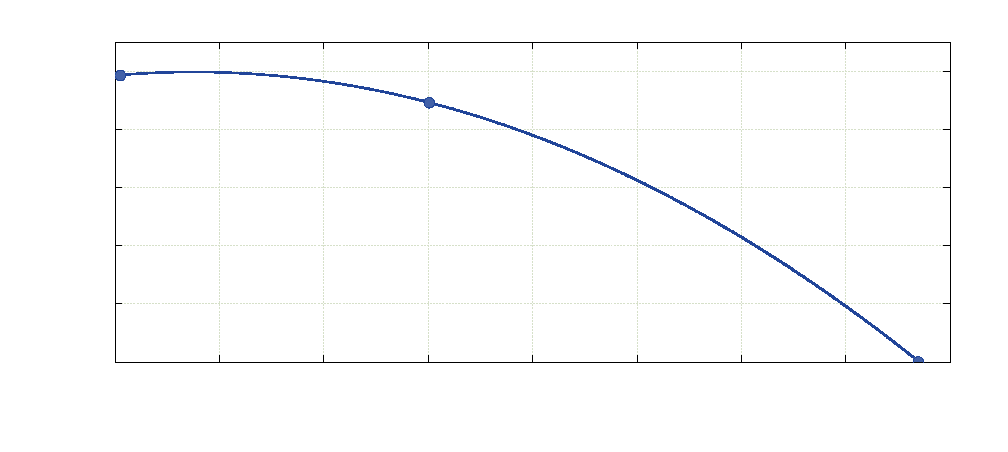
\includegraphics{Graphs/3/AproxCurve/AproxCurve}}%
    \gplfronttext
  \end{picture}%
\endgroup
}
			\caption{Estimating the characteristic curve of a compressor by fitting a quadratic function to points of operation.}
			\label{fig: Compressor Curve}
		\end{figure}

		\par
		Once the models are accurately calibrated, the compressor component is integrated to the air network in the arrangement shown in figure \ref{fig: Compressor models}. The Compressor is connected to the inlet air source via an inlet pipe and air node and to the rest of the network via an air node and outlet pipe. This is is to allow the inlet and outlet parameters and conditions to be be monitored and controlled.
		\begin{figure}[h]
			\centering
			\fbox{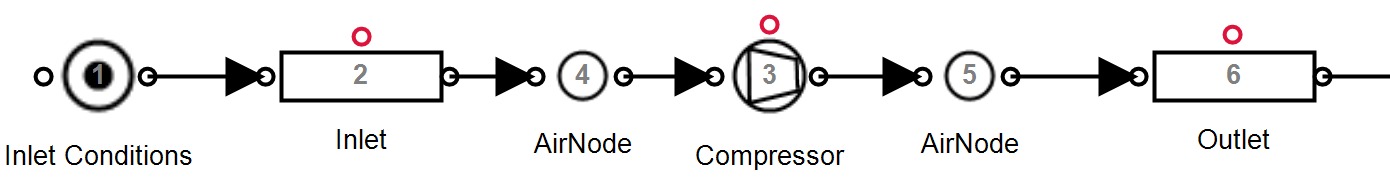
\includegraphics[trim =-4cm 0 -4cm 0cm, width=\textwidth]{Images/3/Compressors}}
			\caption{Integrating the compressor component into the simulation.}
			\label{fig: Compressor models}
		\end{figure}		

		\subsubsection{Demand/leak}
			A flow demand represents any air flow leaving the network. This includes equipment that uses air such as drills and agitators etc. as well as inefficiencies like leaks and open pipes. Generally  the air flow to dependant on pressure and the specific resistance to flow of the outlet. 
			\par 
			The specific resistance of the flow demand can be obtained using the inlet pressure, outlet pressure and flow. If the flow is not known, a reasonably accurate estimation can be made by calculating the expected flow from the size of the outlet.
		\subsubsection{Compressed air control}\label{Controllers}
			Simulation components need to be dynamically controlled as in the actual air network. Control is typically implemented on compressors and valves throughout the network to follow certain set-points and schedules. It is important to not only include the controllers in the simulation, but to replicate the non-linearities, limitations and responsiveness related to their use. This ensures the model reacts in the same way the actual network would, improving accuracy.
			\par 
			On a typical mine, compressors power is controlled to ensure that the discharge pressure matches a specified set-point. This control is achieved through either \glspl{vsd} (or \glspl{vfd}) and guide-vain control. \glspl{vfd} gives a wide range of power control and can be estimated using a \gls{pi} controller as in figure \ref{fig: Controller models} where discharge pressure is used as feedback for the controller. 
	\begin{figure}[h]
		\centering
		\fbox{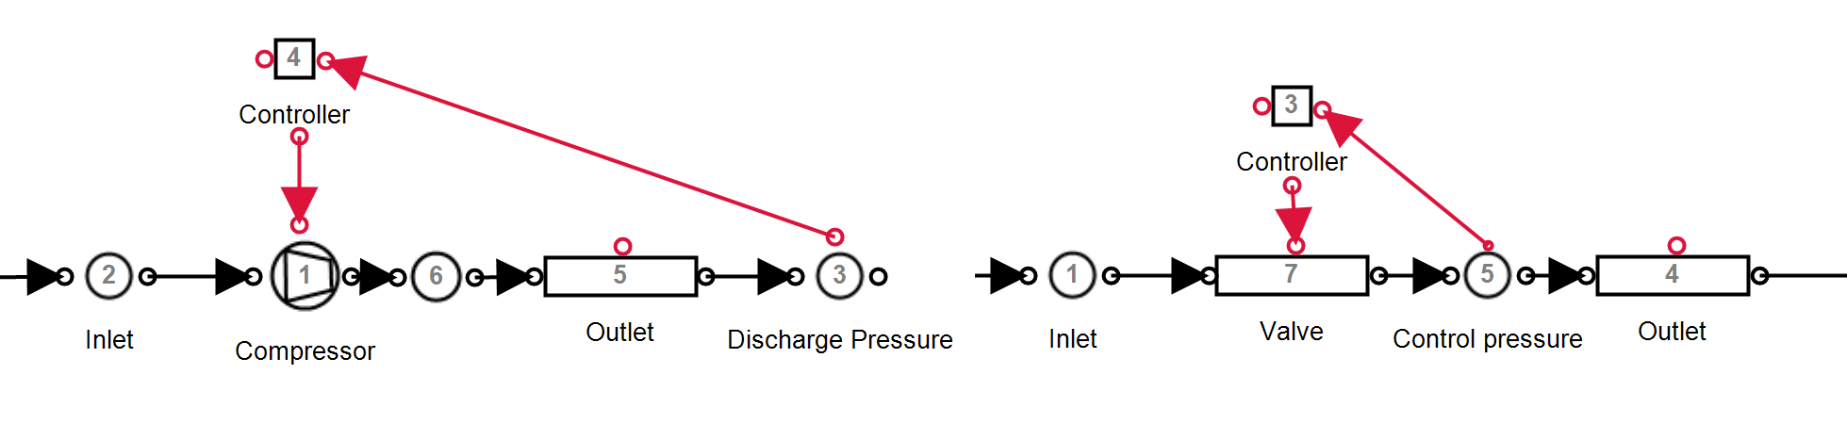
\includegraphics[trim =-4cm 0 -4cm 0cm, width=\textwidth]{Images/3/Controller}}
		\caption{Control components in \gls{stb}.}
		\label{fig: Controller models}
	\end{figure}
	\subsubsection{Compressed air control}
		On many large compressed air networks, the intake guide vain position on a compressor is controlled. Typically, a guide vain is opened or closed to control the compressors discharge pressure.  Manipulating the guide vain position will effect the power of the compressor. The relationship between power and guide vain position of a compressor can be approximated as a linear function. A guide vain position of 40\% will map to an output power of about 60\% of the maximum power. When more pressure is required than can be obtained with the guide vains fully opened, another compressor is needed to operate. Figure \ref{fig: Guide vain position} shows the trend of output power of a compressor vs. inlet guide vain position.
		\begin{figure}[h]
			\centering
			\fbox{% GNUPLOT: LaTeX picture with Postscript
\begingroup
  \makeatletter
  \providecommand\color[2][]{%
    \GenericError{(gnuplot) \space\space\space\@spaces}{%
      Package color not loaded in conjunction with
      terminal option `colourtext'%
    }{See the gnuplot documentation for explanation.%
    }{Either use 'blacktext' in gnuplot or load the package
      color.sty in LaTeX.}%
    \renewcommand\color[2][]{}%
  }%
  \providecommand\includegraphics[2][]{%
    \GenericError{(gnuplot) \space\space\space\@spaces}{%
      Package graphicx or graphics not loaded%
    }{See the gnuplot documentation for explanation.%
    }{The gnuplot epslatex terminal needs graphicx.sty or graphics.sty.}%
    \renewcommand\includegraphics[2][]{}%
  }%
  \providecommand\rotatebox[2]{#2}%
  \@ifundefined{ifGPcolor}{%
    \newif\ifGPcolor
    \GPcolortrue
  }{}%
  \@ifundefined{ifGPblacktext}{%
    \newif\ifGPblacktext
    \GPblacktextfalse
  }{}%
  % define a \g@addto@macro without @ in the name:
  \let\gplgaddtomacro\g@addto@macro
  % define empty templates for all commands taking text:
  \gdef\gplbacktext{}%
  \gdef\gplfronttext{}%
  \makeatother
  \ifGPblacktext
    % no textcolor at all
    \def\colorrgb#1{}%
    \def\colorgray#1{}%
  \else
    % gray or color?
    \ifGPcolor
      \def\colorrgb#1{\color[rgb]{#1}}%
      \def\colorgray#1{\color[gray]{#1}}%
      \expandafter\def\csname LTw\endcsname{\color{white}}%
      \expandafter\def\csname LTb\endcsname{\color{black}}%
      \expandafter\def\csname LTa\endcsname{\color{black}}%
      \expandafter\def\csname LT0\endcsname{\color[rgb]{1,0,0}}%
      \expandafter\def\csname LT1\endcsname{\color[rgb]{0,1,0}}%
      \expandafter\def\csname LT2\endcsname{\color[rgb]{0,0,1}}%
      \expandafter\def\csname LT3\endcsname{\color[rgb]{1,0,1}}%
      \expandafter\def\csname LT4\endcsname{\color[rgb]{0,1,1}}%
      \expandafter\def\csname LT5\endcsname{\color[rgb]{1,1,0}}%
      \expandafter\def\csname LT6\endcsname{\color[rgb]{0,0,0}}%
      \expandafter\def\csname LT7\endcsname{\color[rgb]{1,0.3,0}}%
      \expandafter\def\csname LT8\endcsname{\color[rgb]{0.5,0.5,0.5}}%
    \else
      % gray
      \def\colorrgb#1{\color{black}}%
      \def\colorgray#1{\color[gray]{#1}}%
      \expandafter\def\csname LTw\endcsname{\color{white}}%
      \expandafter\def\csname LTb\endcsname{\color{black}}%
      \expandafter\def\csname LTa\endcsname{\color{black}}%
      \expandafter\def\csname LT0\endcsname{\color{black}}%
      \expandafter\def\csname LT1\endcsname{\color{black}}%
      \expandafter\def\csname LT2\endcsname{\color{black}}%
      \expandafter\def\csname LT3\endcsname{\color{black}}%
      \expandafter\def\csname LT4\endcsname{\color{black}}%
      \expandafter\def\csname LT5\endcsname{\color{black}}%
      \expandafter\def\csname LT6\endcsname{\color{black}}%
      \expandafter\def\csname LT7\endcsname{\color{black}}%
      \expandafter\def\csname LT8\endcsname{\color{black}}%
    \fi
  \fi
    \setlength{\unitlength}{0.0500bp}%
    \ifx\gptboxheight\undefined%
      \newlength{\gptboxheight}%
      \newlength{\gptboxwidth}%
      \newsavebox{\gptboxtext}%
    \fi%
    \setlength{\fboxrule}{0.5pt}%
    \setlength{\fboxsep}{1pt}%
\begin{picture}(9360.00,4032.00)%
    \gplgaddtomacro\gplbacktext{%
      \colorrgb{0.00,0.00,0.00}%
      \put(814,704){\makebox(0,0)[r]{\strut{}$0$}}%
      \colorrgb{0.00,0.00,0.00}%
      \put(814,1214){\makebox(0,0)[r]{\strut{}$20$}}%
      \colorrgb{0.00,0.00,0.00}%
      \put(814,1725){\makebox(0,0)[r]{\strut{}$40$}}%
      \colorrgb{0.00,0.00,0.00}%
      \put(814,2235){\makebox(0,0)[r]{\strut{}$60$}}%
      \colorrgb{0.00,0.00,0.00}%
      \put(814,2746){\makebox(0,0)[r]{\strut{}$80$}}%
      \colorrgb{0.00,0.00,0.00}%
      \put(814,3256){\makebox(0,0)[r]{\strut{}$100$}}%
      \colorrgb{0.00,0.00,0.00}%
      \put(814,3767){\makebox(0,0)[r]{\strut{}$120$}}%
      \colorrgb{0.00,0.00,0.00}%
      \put(946,484){\makebox(0,0){\strut{}$0$}}%
      \colorrgb{0.00,0.00,0.00}%
      \put(2282,484){\makebox(0,0){\strut{}$20$}}%
      \colorrgb{0.00,0.00,0.00}%
      \put(3618,484){\makebox(0,0){\strut{}$40$}}%
      \colorrgb{0.00,0.00,0.00}%
      \put(4954,484){\makebox(0,0){\strut{}$60$}}%
      \colorrgb{0.00,0.00,0.00}%
      \put(6290,484){\makebox(0,0){\strut{}$80$}}%
      \colorrgb{0.00,0.00,0.00}%
      \put(7626,484){\makebox(0,0){\strut{}$100$}}%
      \colorrgb{0.00,0.00,0.00}%
      \put(8962,484){\makebox(0,0){\strut{}$120$}}%
    }%
    \gplgaddtomacro\gplfronttext{%
      \csname LTb\endcsname%
      \put(176,2235){\rotatebox{-270}{\makebox(0,0){\strut{}Output power (\%)}}}%
      \put(4954,154){\makebox(0,0){\strut{}Guide Vain Position (\%)}}%
    }%
    \gplbacktext
    \put(0,0){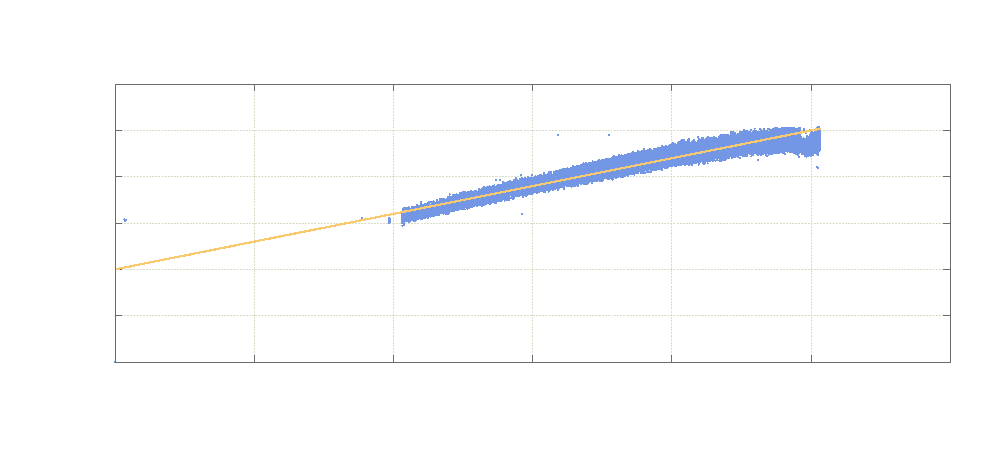
\includegraphics{Graphs/1/GuideVainPosition/GuideVainPosition}}%
    \gplfronttext
  \end{picture}%
\endgroup
}
			\caption[The relation between guide vain position and compressor output power.]{The relation between guide vain position and compressor output power.}
			\label{fig: Guide vain position}
		\end{figure}
		\par
		A guide vain controller is modelled using a \gls{pi} controller, as with the \gls{vsd} controller. However the limitations of guide vain control, as shown in figure \ref{fig: Guide vain position}, must be implemented to the controller. This is implemented by using a minimum output that would match the minimum power reduction fraction the guide vain achieved by closing the guide vain. For example, a \gls{pi} control for the compressor from figure \ref{fig: Guide vain position} would have a minimum control output of approximately 60\%.
		\par 
		Mines utilise control valves underground sections to control the pressure at individual mining stations independently \cite{Heyns2014Masters}. Controlling of valve components is perfomed similarly as control of the compressor components. As shown in figure \ref{fig: Controller models} the outlet pressure is used as feedback for a pi controller. The controller output is mapped to the valve fraction of a pipe component.
		\begin{figure}[h]
			\centering
			\fbox{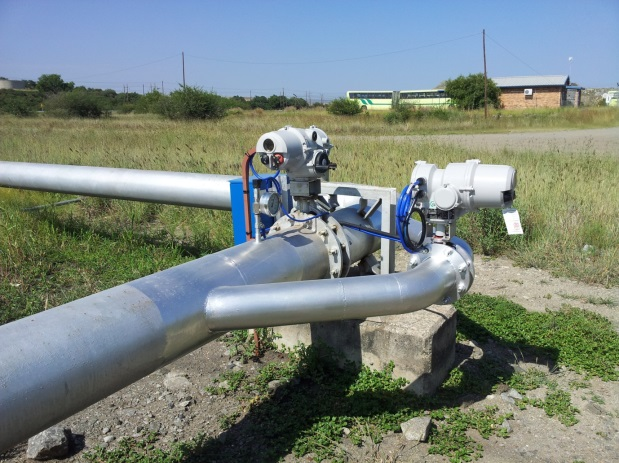
\includegraphics[trim =-4cm 0 -4cm 0cm, width=\textwidth]{Images/3/Valve.jpg}}
			\caption[An example of a compressed air control valve.]{An example of a compressed air control valve\cite{van2015implementation}.} 
			\label{fig: Control}
		\end{figure}
		\subsubsection{Compressed air after-cooling}
		The air compression process generates significant heat. Compressed air at high temperatures contains a large amount of water vapour. To prevent condensation later in the air network, improve the system capacity and protect equipment from excessive heat, after-coolers are installed to the outlet of the compressor \cite{schroeder2009energy}.
		\par 
		After-cooling reduces the compressed air temperature to within a margin of ambient. This cooling could have a large effect on the performance of the network. Hence including after-cooling to the simulation model should improve accuracy.
		\par 
		To replicate this effect, a heat transfer node can be added to the outlet of the compressor component. \gls{stb} utilizes the following heat transfer parameters of the air node to solve for outlet temperature:
		\par 
		\begin{tabular}{p{1.3cm}p{13cm}}
			$Area$ & The heat transfer area ($m^2$) \\
			$UA$ & Heat transfer coefficient ($kW/^{\circ} C$) \\
			$T_{amb}$ & Ambient air temperature ($^{\circ} C$) \\
		\end{tabular} \\	
	\subsection{Simulation inputs}
		- Discuss inputs of the simulation, (compressor setpoints, ambient conditions, demands)
	\subsection{Verification of simulation model}
		- Steps to validate  the model accuracy .\\
		- Compare parameters to actuals\\
		- First principles\\
		-
	\subsection{Summary}
\section{Implementation of simulation method}
	\subsection{Preamble}
		Once a simulation has been developed and verified, the implementation of interventions and scenarios follows. In this section, the approach of implementation, and analysis of interventions in simulation will be discussed.
	\subsection{Analyses of data}
		- Baseline vs Optimised comparison \\
	\subsection{Quantifying operational improvements}
		- Estimating cost savings
	\subsection{Summary}
\section{Conclusion}
